\documentclass[runningheads,a4paper]{llncs}

\usepackage[T1]{fontenc}
\usepackage[utf8]{inputenc}
\usepackage{lmodern}
\usepackage{graphicx}
\usepackage{amsmath}
\usepackage{amssymb}
\usepackage{booktabs}
\usepackage{array}
\usepackage{url}
\usepackage[hypertexnames=false,hidelinks]{hyperref}
\usepackage{placeins}
\usepackage{algorithm}
\usepackage{algorithmic}

\setlength{\textfloatsep}{7pt plus 2pt minus 2pt}
\setlength{\floatsep}{6pt plus 2pt minus 2pt}
\setlength{\intextsep}{6pt plus 2pt minus 2pt}
\setlength{\abovecaptionskip}{3pt}
\setlength{\belowcaptionskip}{0pt}
\setlength{\abovedisplayskip}{5pt plus 1pt minus 1pt}
\setlength{\belowdisplayskip}{5pt plus 1pt minus 1pt}
\emergencystretch=1.5em

\begin{document}

\title{No-PWM Power Estimation for Fixed-Wing UAVs: A Rolling GRU Baseline with Preliminary Attribution and Flight-Level Energy Indicators}

\titlerunning{No-PWM GRU UAV Power Baseline}

\author{Thu Le\inst{1,2,3} \and Hoang Duc Tai\inst{3} \and Nhat Truong\inst{3}}

\authorrunning{T. Le et al.}

\institute{Faculty of Information Technology, University of Science, Ho Chi Minh City, Vietnam \and
Vietnam National University, Ho Chi Minh City, Vietnam \and
FPT University, Ho Chi Minh City, Vietnam\\
\email{thulvm@fpt.edu.vn, ductaiph810@gmail.com, truong16102006@gmail.com}}

\maketitle

\begin{abstract}
Fixed-wing UAV operators need reliable power estimates to plan charging, review missions, and detect unusual energy use. Many flight logs contain highly predictive signals such as PWM, actuator commands, voltage, current, or route identifiers. These signals, however, may be unavailable, platform specific, delayed, or too close to the target mechanism for a conservative state-based benchmark. This study evaluates whether instantaneous electrical power can be estimated from vehicle state and causal time context alone after those channels are removed. The objective is not to replace actuator-aware models, but to define a leakage-audited reference task for incomplete or heterogeneous telemetry. Using a cleaned IDF DS subset with 60,454 samples, 118 flights, and seven chronological campaigns, we train and evaluate sequence models under strict rolling future validation. The selected GRU reaches aggregate RMSLE 0.2588, RMSE 22.99\,W, and $R^2 = 0.8704$ across C4--C7, with flight-bootstrap RMSLE 95\% CI [0.2445, 0.2730]. The result is not uniform: C7 exposes a serious failure mode, with RMSE 54.32\,W. The same held-out predictions are further used for flight-level Wh aggregation, preliminary SHAP-based attribution, and a lightweight C7 adaptation check. These diagnostics connect point prediction with operational review by estimating energy bands, identifying plausible state drivers, and indicating when recalibration is needed. The contribution is a transparent no-PWM baseline, together with evidence on when this state-only approach works, when it fails, and how it can support human-reviewed UAV energy audits.

\keywords{UAV telemetry \and instantaneous power regression \and GRU \and no-PWM baseline \and preliminary attribution \and rolling validation}
\end{abstract}

%------------------------------------------------------------------------
\section{Introduction}

Energy availability is a central constraint for small UAVs. Shakhatreh et al.\ identify endurance, payload, safety, communication, and onboard resources as deployment barriers for civil UAV applications~\cite{shakhatreh2019survey}. Mozaffari et al.\ frame these constraints in UAV communication and networking systems, where energy limits shape coverage and service continuity~\cite{mozaffari2019tutorial}. Hayat et al.\ emphasize that endurance and energy-aware coordination remain operational concerns in multi-UAV settings~\cite{hayat2016survey}. In fixed-wing missions, power depends on airspeed, climb and sink behavior, attitude, acceleration, air density, wind, and phase. Energy cost is tied to trajectory choices in UAV communication models~\cite{zeng2017energy}, coverage constraints in aerial imaging missions~\cite{difranco2016coverage}, and battery behavior in access-network deployments~\cite{abeywickrama2018access}. Learning-based energy models motivate data-driven estimation from flight logs~\cite{gora2022ml}. Broader drone-model comparisons reinforce the same need for empirical prediction while showing that assumptions differ across platforms and tasks~\cite{zhang2021models}. Together, this literature raises a methodological issue: the most predictive logged variables are not always appropriate inputs for a deployment-oriented benchmark.

Here the practical issue is the no-PWM setting. PWM, actuator channels, throttle variables, voltage, and current are informative in retrospective logs, but may be unavailable, platform dependent, noisy, delayed, or too close to the target mechanism. A model that depends on them may report strong accuracy without showing that power can be inferred from vehicle state itself. We define the target as instantaneous electrical power,
\begin{equation}
  P_t = \texttt{power\_w}(t), \quad P_t \; [\mathrm{W}], \label{eq:target}
\end{equation}
where $t$ is the telemetry timestamp. The focus is whether a leakage audited state time representation can provide a credible baseline without PWM.

The IDF DS benchmark provides 240 fixed-wing autonomous missions and more than 32 hours of telemetry~\cite{garcia2026idfds}; its descriptor does not train or evaluate a neural power predictor. We use this gap to audit neural instantaneous power prediction on a cleaned 118-flight subset while removing PWM, actuator, electrical, and route-identifying information. We ask whether state time sequence models form a credible no-PWM baseline, whether rolling validation exposes shift more honestly than shuffled references, whether a PWM-aware ablation quantifies the feature-policy cost, and whether GRU explanations identify plausible state drivers.

UAV deployments require energy-aware coordination across vehicles and missions~\cite{hayat2016survey}. They also require safety and security assurance because logged control channels may be operationally sensitive or platform dependent~\cite{yaacoub2020security}. We exclude route identifiers, actuator commands, and platform-specific electrical fields to test what can be inferred from vehicle state alone, not to assert a separate PWM-privacy claim.

The main contribution is a leakage audited no-PWM regression baseline validated by strict rolling future campaigns. Secondary diagnostics translate the same held-out predictions into flight-level energy indicators and preliminary attribution evidence. We deliberately report both aggregate performance and failure analysis because a useful operational model must reveal when its assumptions stop holding. The selected backbone is a GRU, using gated recurrence introduced for compact sequence modeling~\cite{cho2014gru}. LSTM provides the longer-established recurrent reference~\cite{hochreiter1997lstm}. TCN supplies a causal fixed-window sequence alternative~\cite{bai2018tcn}. DeepAR motivates future probabilistic forecasting extensions rather than serving as a direct baseline here~\cite{salinas2020deepar}. Temporal attention models motivate richer future sequence explanations and uncertainty modeling~\cite{lim2021tft}. Time-series reviews motivate careful benchmark design for sequence learning~\cite{fawaz2019dlts}. Validation literature motivates chronological evaluation rather than shuffled testing~\cite{bergmeir2018cv}. Leakage studies justify the conservative feature policy~\cite{kaufman2012leakage}. Drone-energy analysis connects Wh estimates to operational planning~\cite{stolaroff2018drone}. SHAP provides the attribution mechanism used for local audit evidence~\cite{lundberg2017shap}. Broader XAI surveys frame those attributions as explanations to be bounded and validated, not causal proof~\cite{arrieta2020xai}.

%------------------------------------------------------------------------
\section{Related Work and Research Positioning}

\begin{table}[!htbp]
\caption{Five focal related works and the position of the proposed no PWM state time benchmark.}
\label{tab:related}
\centering
{\scriptsize
\renewcommand{\arraystretch}{0.84}
\begin{tabular}{p{1.0cm} p{2.1cm} p{3.9cm} p{3.9cm}}
\toprule
Item & Focal paper & Main content & Position in this paper \\
\midrule
Article 1 & Shakhatreh et al.\ \cite{shakhatreh2019survey} &
  Civil UAV applications; endurance, safety, communication, payload, and onboard resource barriers. &
  Motivates deployment oriented power prediction for UAV operations. \\[1pt]
Article 2 & Zeng and Zhang \cite{zeng2017energy} &
  Energy efficient UAV communication and trajectory optimization. &
  Supports state, air data, and causal time as energy predictors after PWM and electrical fields are removed. \\[1pt]
Article 3 & Garcia-Gascon et al.\ \cite{garcia2026idfds} &
  IDF DS: 240 fixed wing missions and more than 32\,h of telemetry. &
  Provides the dataset gap: no neural power predictor is trained in the descriptor. \\[1pt]
Article 4 & Lundberg and Lee \cite{lundberg2017shap} &
  SHAP feature attribution for model explanations. &
  Explains the selected GRU directly, rather than using SHAP as a baseline model. \\[1pt]
Article 5 & Hochreiter and Schmidhuber \cite{hochreiter1997lstm}; Cho et al.\ \cite{cho2014gru} &
  Recurrent sequence models for temporal representation learning. &
  Motivates LSTM and GRU as neural references for the no PWM sequence task. \\
\bottomrule
\end{tabular}
}
\end{table}

TCNs provide causal fixed-window sequence modeling~\cite{bai2018tcn}, while LSTM~\cite{hochreiter1997lstm} and GRU~\cite{cho2014gru} provide recurrent alternatives. DeepAR represents probabilistic autoregressive forecasting and motivates future uncertainty-aware comparisons~\cite{salinas2020deepar}. Temporal attention models motivate future work on interpretable multi-horizon sequence prediction~\cite{lim2021tft}. Time-series reviews motivate careful neural benchmark design~\cite{fawaz2019dlts}. Leakage studies motivate removing variables that encode the target or future information too directly~\cite{kaufman2012leakage}. Validation work motivates chronological testing rather than shuffled splits~\cite{bergmeir2018cv}.

Drone energy evidence connects flight-level Wh estimates to logistics planning~\cite{stolaroff2018drone}. SHAP supplies the feature-attribution mechanism used for local model auditing~\cite{lundberg2017shap}. XAI surveys support treating attribution as bounded audit evidence, not causal proof~\cite{arrieta2020xai}. The study therefore has one main contribution and two supporting diagnostics: rolling no-PWM prediction, preliminary GradientExplainer/permutation evidence, and flight-level energy indicators.

%------------------------------------------------------------------------
\section{Materials and Methods}

\subsection{Dataset and Chronological Partition}

We use \texttt{dataset\_timeseries\_cleaned\_v2.csv}, derived from the public IDF DS Holybro/Pixhawk telemetry released on Zenodo~\cite{garcia2025zenodo} and described in \textit{Scientific Data}~\cite{garcia2026idfds}. The full benchmark has 240 flights; our cleaned fixed-wing autonomous subset starts from 120 flights, 60,512 telemetry rows, and 3,003 raw signal columns. After timestamp correction, removal of two incomplete flights and 42 nonpositive-power rows, the retained table has 60,454 rows, 33 retained columns, 118 flights, zero missing entries, and median sampling interval 0.506\,s. Seven chronological campaigns are derived from flight order. PWM and throttle fields remain in the CSV for traceability but are excluded from every model reported here.

Figure~\ref{fig:workflow} links cleaning provenance, the no-PWM feature contract, causal state time construction, model scoring, and diagnostics to rolling future validation. C1--C3 form development; C4--C7 are future tests trained only on earlier campaigns.

\begin{figure}[!htbp]
  \centering
  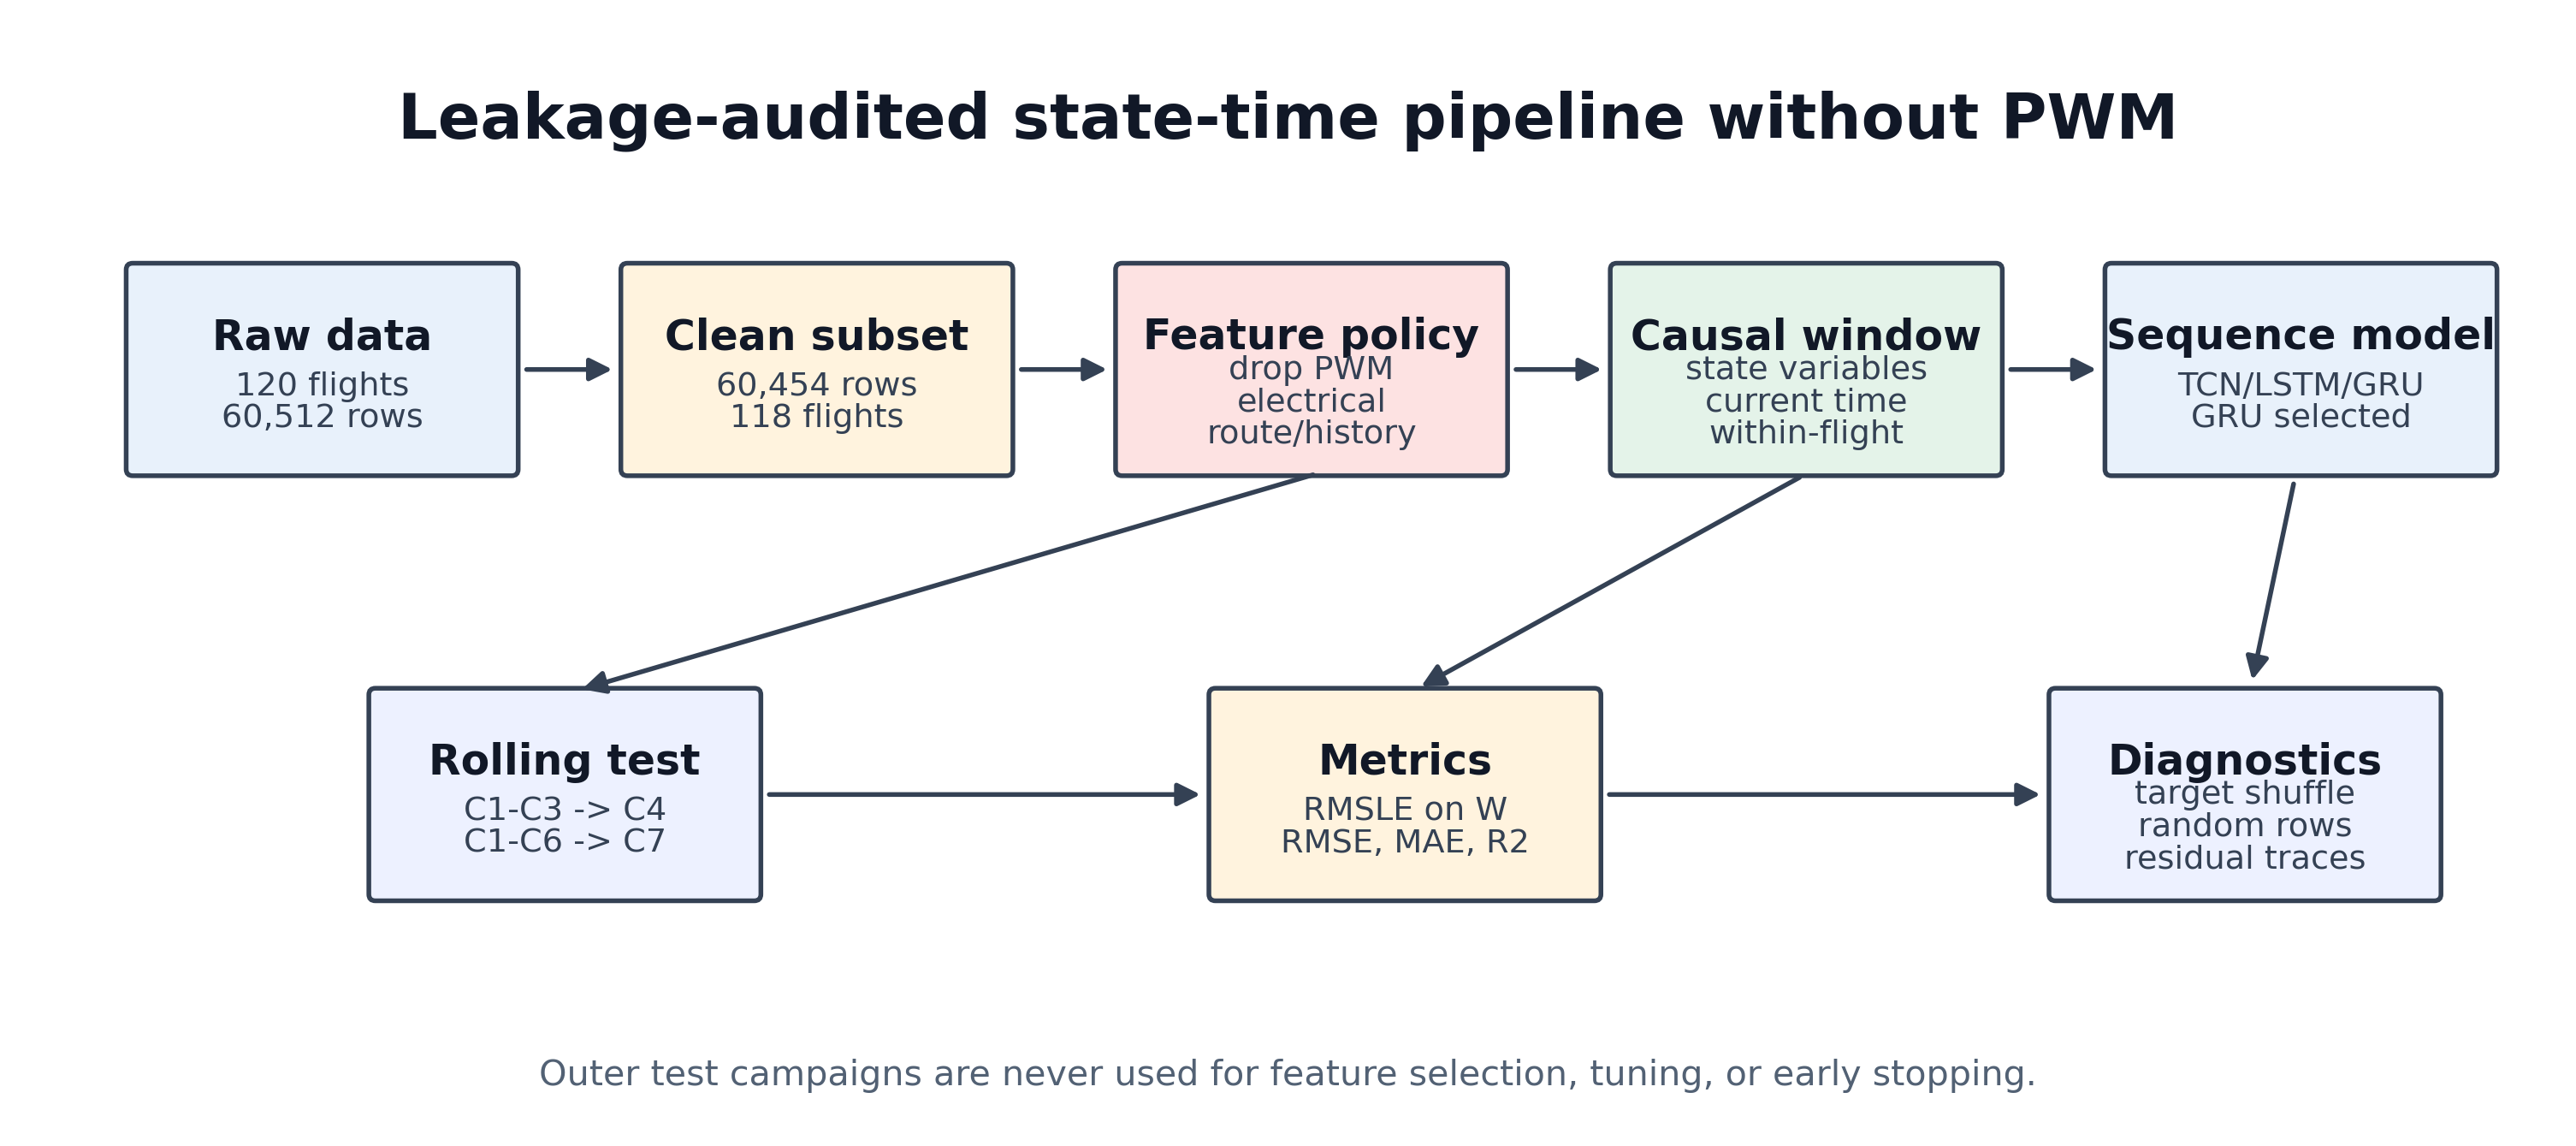
\includegraphics[width=0.80\textwidth]{lncs_figures/idf_state_time_workflow.png}
  \caption{End to end state time workflow used to construct and evaluate the power regression benchmark without PWM.}
  \label{fig:workflow}
\end{figure}

Figure~\ref{fig:data} verifies the retained quantities: 118 flights, 60,454 records, mean power 136.47\,W, median power 152.38\,W, and maximum power 311.29\,W. C7 has the highest mean power; phase averages show climb, level, and descent in the expected order. The figure is used as a dataset audit rather than a modeling result, so the campaign and phase summaries are descriptive checks on the retained subset before any future folds are evaluated.

\begin{figure}[!htbp]
  \centering
  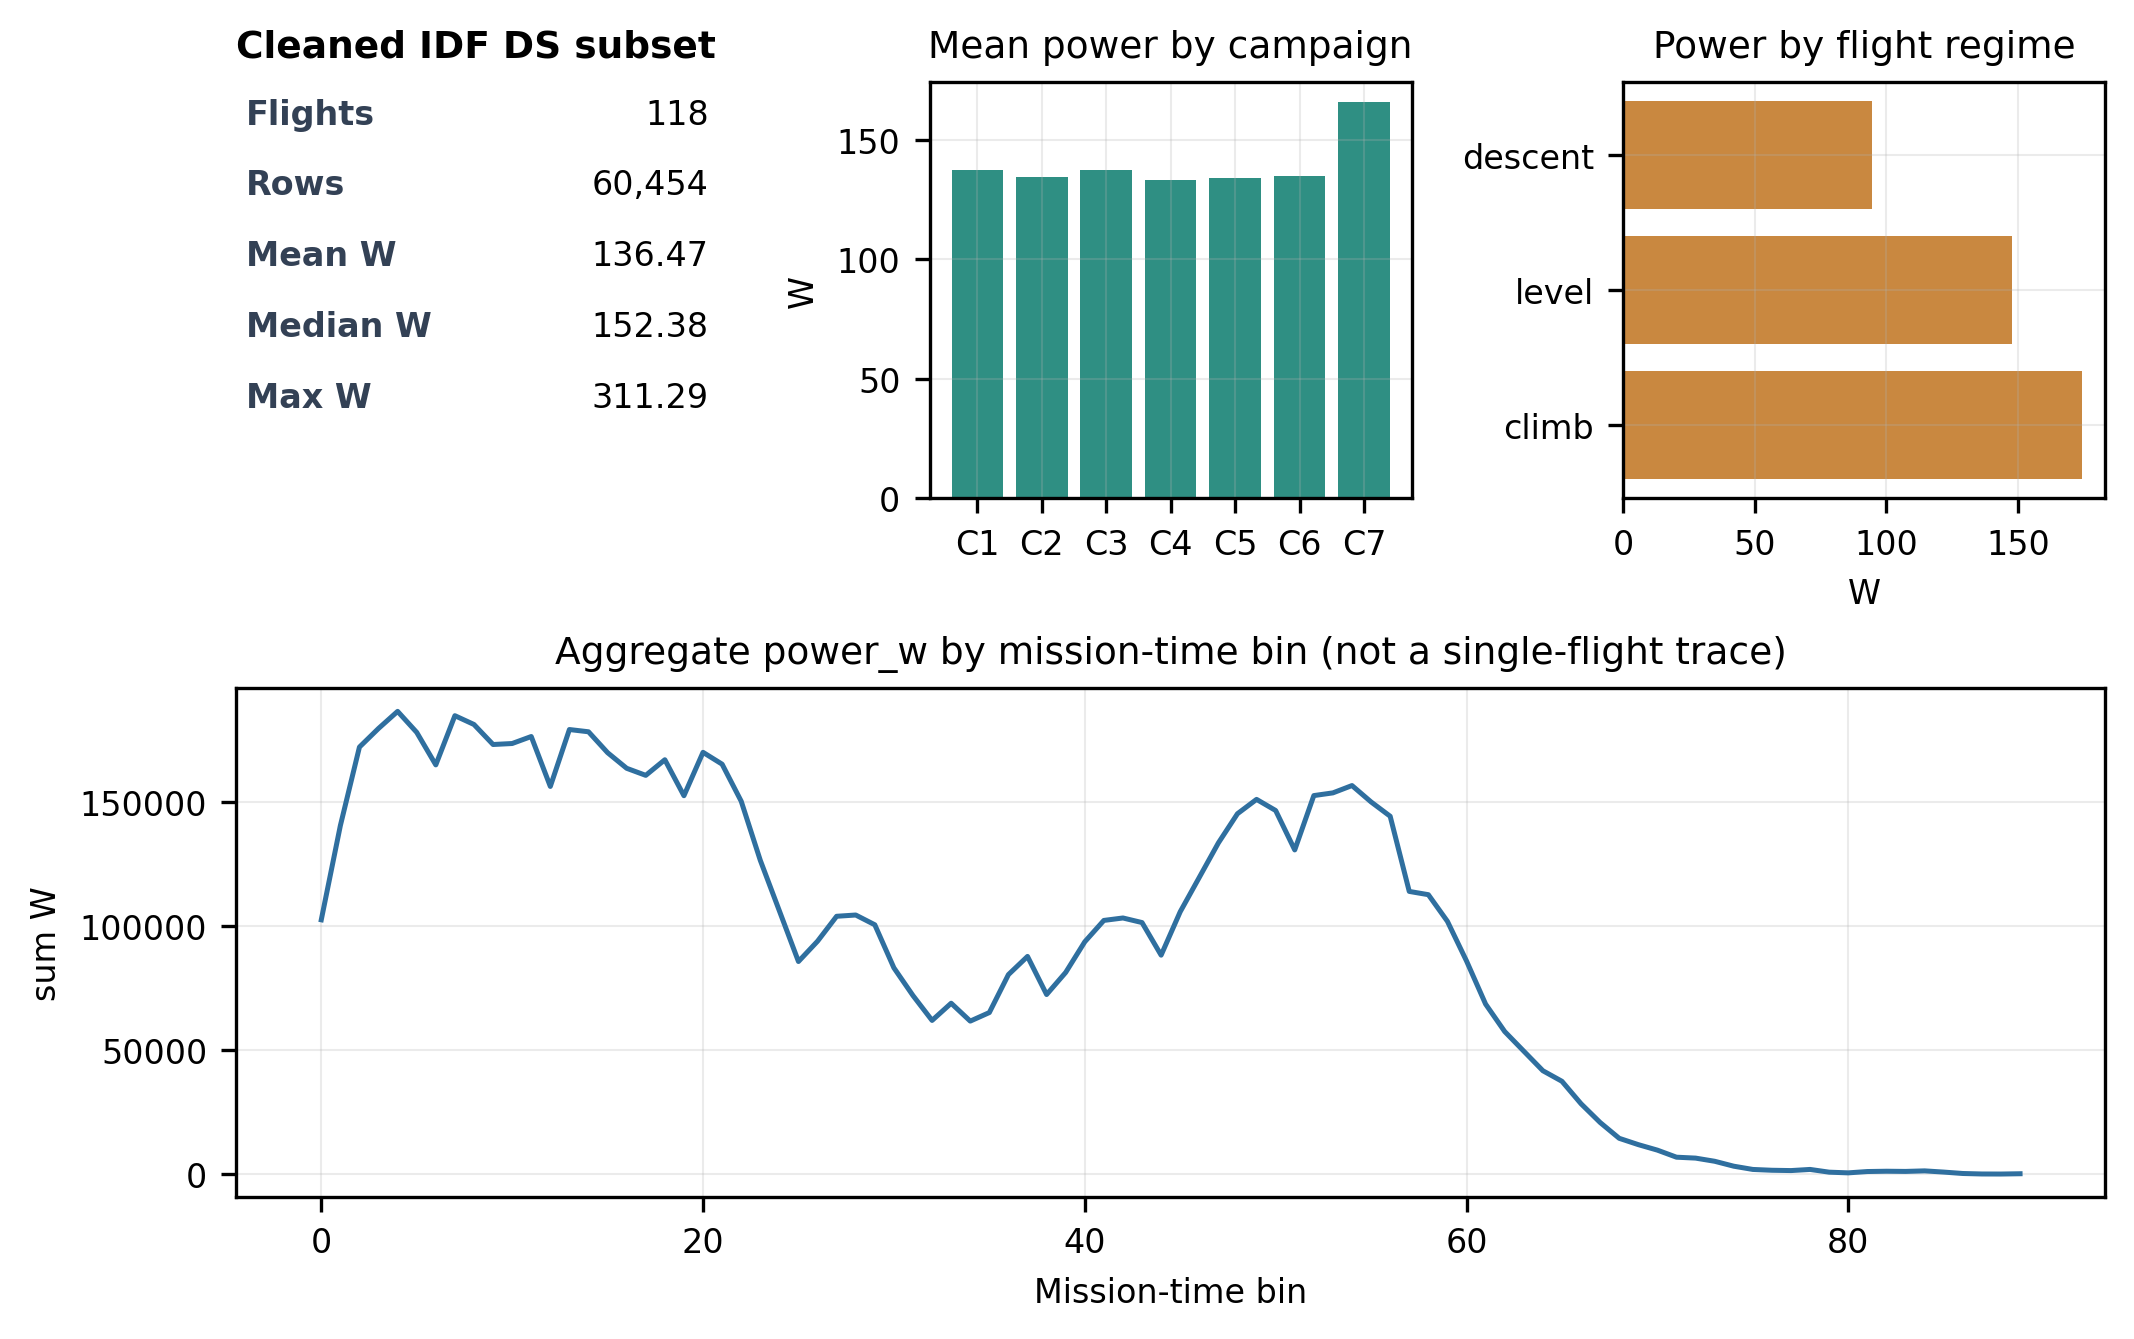
\includegraphics[width=0.64\textwidth]{lncs_figures/idf_dataset_overview_vector.png}
  \caption{Cleaned IDF DS subset used by the no-PWM benchmark. The panels report retained flights and records, the empirical power distribution, campaign-level mean power, phase-level mean power, and an aggregate mission-time trace. The trace is a binned sum of \texttt{power\_w} over all retained flights, included only to show temporal coverage and scale; it is not a single-flight trajectory or a future-test prediction.}
  \label{fig:data}
\end{figure}
\FloatBarrier

\subsection{State Time Feature Policy}

The feature policy separates telemetry state from leakage-prone or deployment-fragile signals. Allowed variables include velocity, acceleration, speed, climb rate, roll, pitch, tilt, air density, temperature, airspeed, wind, headwind, derived physical quantities, current \texttt{t\_sec}, elapsed/log time, and fixed sine/cosine cycles available at prediction time.

Excluded variables are identifiers, campaign labels, \texttt{power\_w}, target histories, motor PWM, throttle, actuator/control channels, voltage, current, battery variables, absolute route coordinates, heading, yaw, centered windows, leads, flight progress, and time-to-end. Elapsed time is observable at $t$; time-to-end is not. Table~\ref{tab:features} summarizes the contract.

\begin{table}[!htbp]
\caption{Feature inventory and leakage controls in the state time pipeline.}
\label{tab:features}
\centering
{\small
\begin{tabular}{lcp{7.0cm}}
\toprule
Group & Count & Interpretation \\
\midrule
Current state time & 40  & Flight dynamics, wind, air data, derived physical quantities, and current timestamp transforms \\
Causal history      & 390 & Shifted lags and rolling statistics computed within the same flight \\
Tabular input       & 430 & Ridge input formed by current state time variables and causal histories \\
Sequence input      & 40  & TCN, LSTM, and GRU per timestep vector in a causal window \\
Time features       & 11  & Current \texttt{t\_sec}, elapsed and log time, and fixed cycle sine/cosine encodings \\
\bottomrule
\end{tabular}
\par\smallskip
\parbox{0.84\textwidth}{\scriptsize All three rows score the same 66 C4--C7 future flights under different review thresholds. The 10.1057\,Wh threshold remains primary because it is fixed from C1--C3 before future testing; 9.0\,Wh is a practitioner-oriented lower threshold when higher recall is preferred.}
}
\end{table}

Ridge receives 430 engineered causal variables; TCN, LSTM, and GRU receive 40-dimensional causal windows. All lag and rolling operations are shifted, so the target timestamp never receives future values.

The association analysis in Fig.~\ref{fig:assoc} is a pre-modeling plausibility check. Pitch, climb behavior, airspeed, dynamic pressure, wind quantities, and time phase variables rank highly, consistent with fixed-wing power intuition. The ranking is descriptive, not causal, and supports the state/time feature policy after actuator and electrical channels are removed.

\begin{figure}[!htbp]
  \centering
  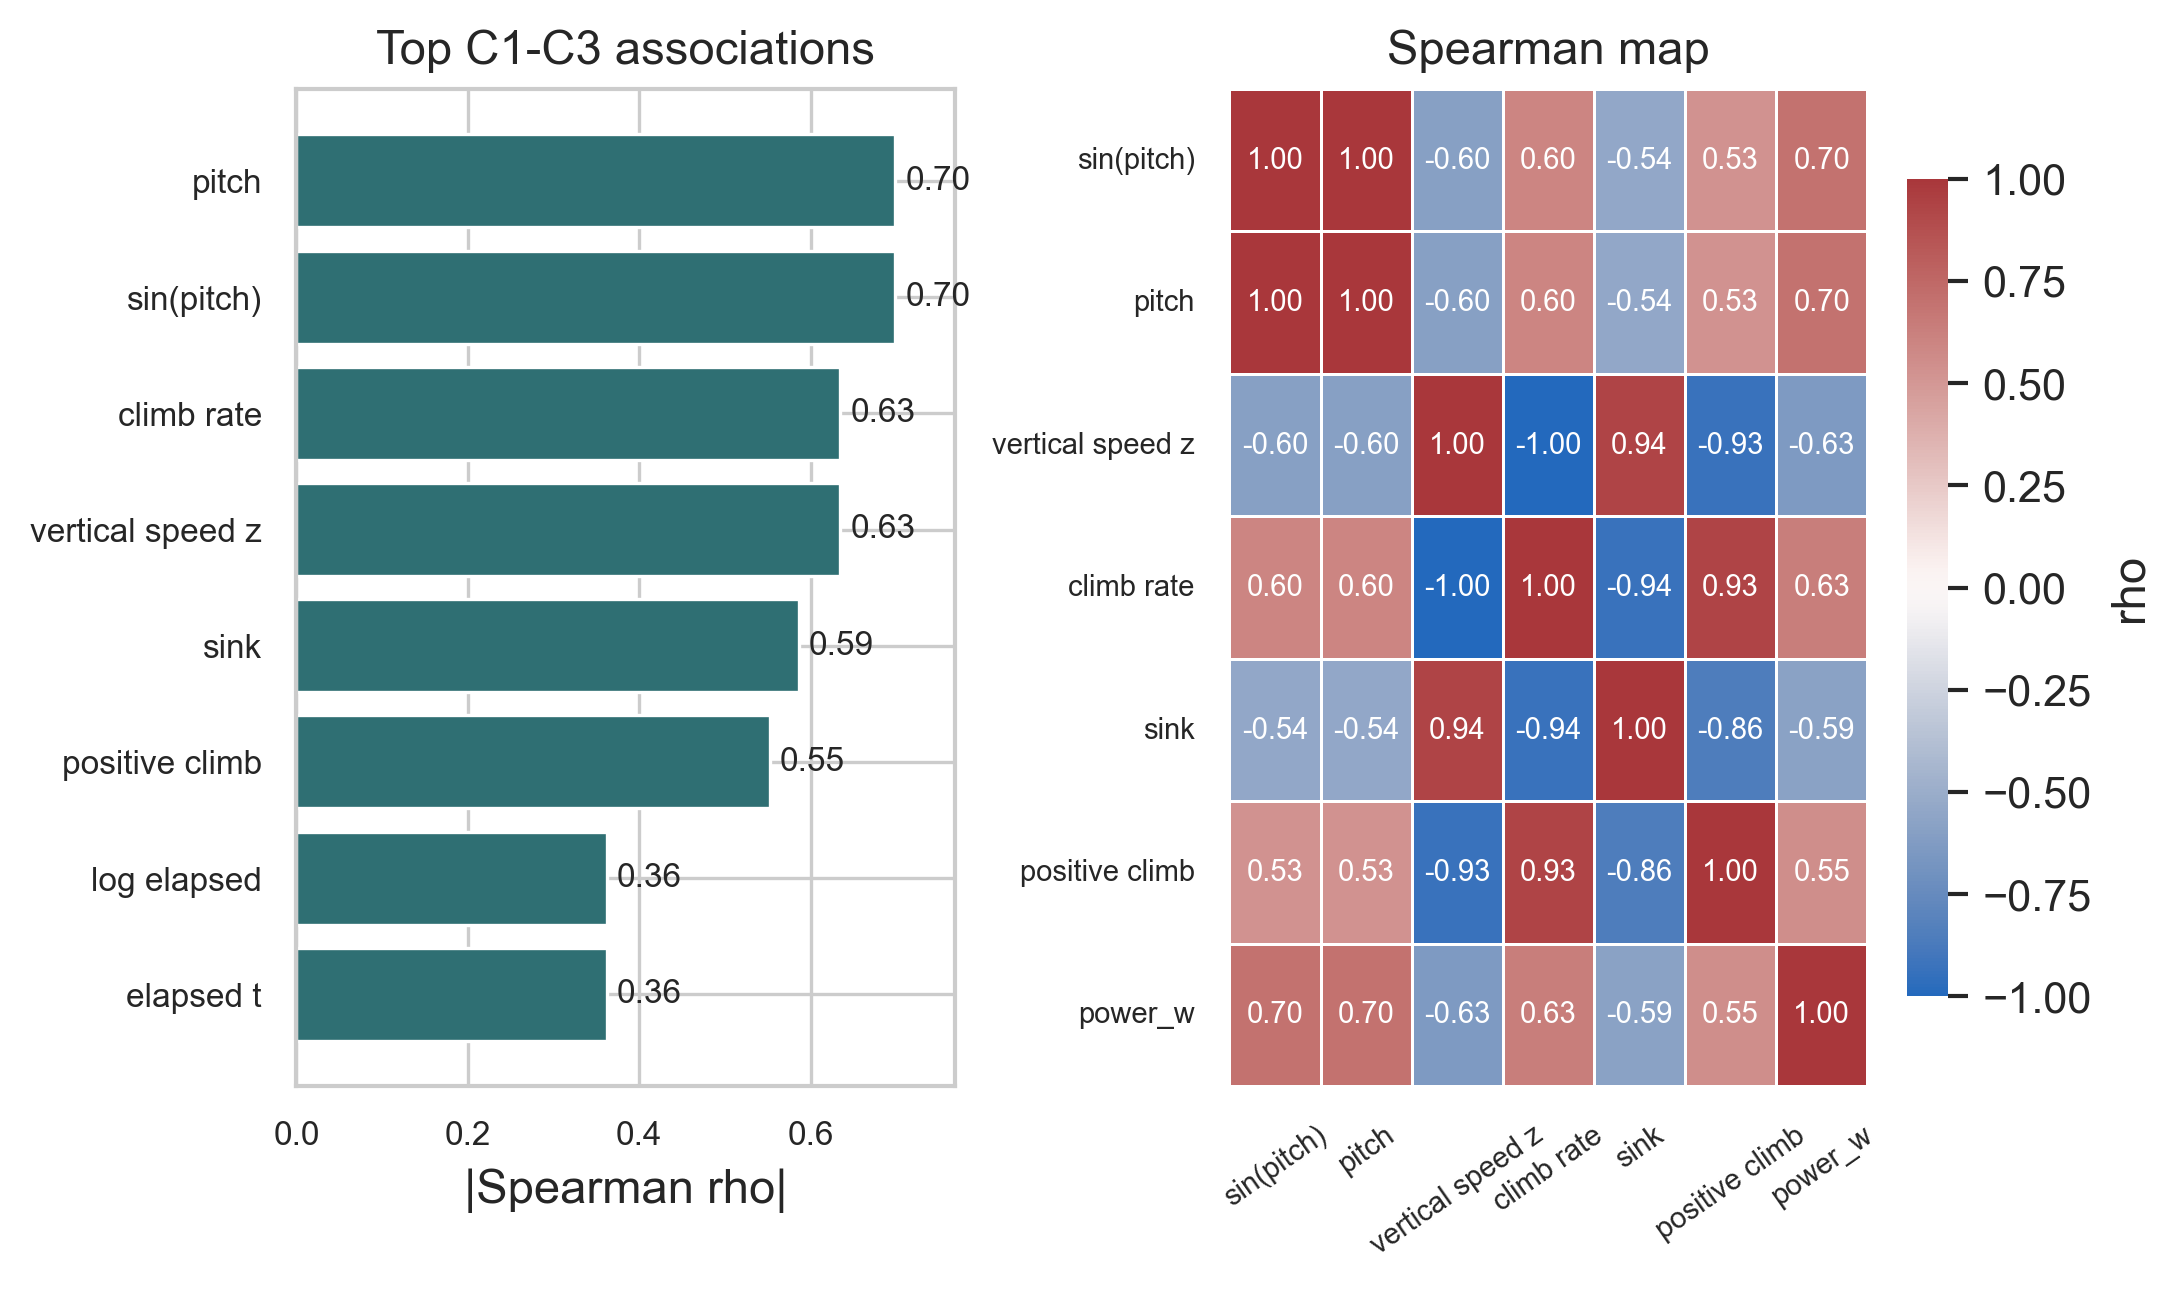
\includegraphics[width=0.90\textwidth]{lncs_figures/state_time_association.png}
  \caption{Association analysis computed only on early campaigns C1 to C3 with enlarged labels for print readability. The ranking is descriptive and is not used to tune future test folds.}
  \label{fig:assoc}
\end{figure}
\FloatBarrier

\subsection{PWM Ablation for Feature Policy}

The no-PWM policy is a benchmark constraint, not an argument that actuator information is uninformative. A PWM-aware ablation with actuator channels available at inference time learns ensemble weights on validation flights 72--89 and freezes them for future flights 90--120. It obtains RMSLE 0.1789, RMSE 17.77\,W, MAE 13.80\,W, $R^2$ 0.9253, and $\Delta R^2$ 0.8561, versus the selected no-PWM GRU's RMSLE 0.2588, RMSE 22.99\,W, MAE 16.78\,W, $R^2$ 0.8704, and $\Delta R^2$ 0.4281.

\begin{table}[!htbp]
\caption{Executed feature-policy ablation. PWM improves accuracy, but the main paper keeps the no-PWM setting as a conservative deployment-oriented benchmark.}
\label{tab:pwmablation}
\centering
{\small
\begin{tabular}{lccccc}
\toprule
Setting & PWM at inference & RMSE\,(W) & MAE\,(W) & RMSLE & $R^2$ \\
\midrule
PWM-aware ablation & Yes & 17.77 & 13.80 & 0.1789 & 0.9253 \\
Selected GRU state time & No & 22.99 & 16.78 & 0.2588 & 0.8704 \\
\bottomrule
\end{tabular}
}
\end{table}

This ablation shows the cost of the exclusion policy: PWM and actuator channels carry strong demand information, so the no-PWM task is harder. The reported contribution is the state-only baseline; the PWM-aware result only makes the trade-off transparent.

\subsection{Causal Feature Engineering and Model}

Derived variables are included for physical interpretability. Dynamic pressure is
\begin{equation}
  q_t = \tfrac{1}{2}\,\rho_t V_t^2, \label{eq:q}
\end{equation}
where $\rho_t$ is air density and $V_t$ is true airspeed. Positive climb/sink split vertical motion, and sine/cosine encodings avoid angular discontinuities. For feature $x_{f,t}$ in flight $f$, causal lags are
\begin{equation}
  x^{(\delta)}_{f,t} = x_{f,t-\delta}, \quad \delta \in \{1,2,3,5,10,20\}. \label{eq:lag}
\end{equation}
Rolling statistics are computed after a one-step shift, so windows ending at $t-1$ predict $P_t$.

Neural references use causal sequence windows. A residual TCN convolution is
\begin{equation}
  h^{(\ell)}_t = \sigma\!\left(\sum_{k=0}^{K-1} W^{(\ell)}_k\, h^{(\ell-1)}_{t - d \cdot k} + b^{(\ell)}\right), \quad d \in \{1,2,4,8\}. \label{eq:tcn}
\end{equation}
where $h^{(0)}_t$ is the 40-variable input and only indices $t-dk\le t$ are used. The TCN has 48 channels, four residual blocks with dilations 1, 2, 4, 8, kernel $K=3$, dropout 0.1, and head $48 \to 24 \to 1$. The physics proxy uses $q_tV_t$, positive climb, positive sink, and clipped $\sec(\mathrm{tilt})$, median imputation, robust 5th--95th percentile scaling, and Ridge $\alpha=30$ on $\log(1+P_t)$; it is a transparent reference, not a full aerodynamic model. The final predictor is selected before C4--C7 by development rolling splits C1$\to$C2 and C1--C2$\to$C3. The selected GRU uses 40 no-PWM inputs, 64-sample causal windows, hidden size 64, two layers, dropout 0.05, head $64 \to 32 \to 1$, AdamW, learning rate $7\times10^{-4}$, weight decay $10^{-4}$, gradient clipping 1.0, 55 epochs, and balanced per-flight weights. The 32-configuration grid covers windows $\{64,96\}$, hidden sizes $\{32,64,96,128\}$, one/two layers, dropout $\{0,0.05\}$, and nearby learning rates; the selected training pass recorded 166\,s locally and no edge-latency claim is made. All neural models use $y_t=\log(1+P_t)$ and $\hat{P}_t=\exp(\hat{y}_t)-1$.

Reported neural numbers come from one audited run with fixed Python, NumPy, and PyTorch seeds, shared rolling folds, and saved artifacts. The local stack was Windows 11, Intel i7-13620H, Python 3.13.7, NumPy 2.4.5, pandas 3.0.3, scikit-learn 1.8.0, Matplotlib 3.10.9, and PyTorch 2.6.0+cu124; flight-cluster bootstrap intervals quantify run-level evidence.

\subsection{Evaluation Protocol}

The outer evaluation is rolling future campaign validation:
\[
  \text{C1 to C3}\to\text{C4},\quad
  \text{C1 to C4}\to\text{C5},\quad
  \text{C1 to C5}\to\text{C6},\quad
  \text{C1 to C6}\to\text{C7}.
\]
All tuning and early stopping use only campaigns prior to the outer test campaign. The primary metric is RMSLE,
\begin{equation}
  \mathrm{RMSLE} = \sqrt{\frac{1}{n}\sum_{i=1}^{n}\bigl[\log(1+\hat{P}_i) - \log(1+P_i)\bigr]^2}. \label{eq:rmsle}
\end{equation}
RMSLE captures relative error and reduces domination by high-power peaks; RMSE and MAE retain watt-scale interpretability, and $R^2$ measures level fit. For the selected GRU, first-difference $R^2$ inspects local temporal changes~\cite{hyndman2006forecast}:
\begin{equation}
  \Delta R^2 = 1 - \frac{\sum_t(\Delta P_t - \Delta\hat{P}_t)^2}{\sum_t(\Delta P_t - \overline{\Delta P})^2}. \label{eq:deltaR2}
\end{equation}
This diagnostic is reported only for selected-GRU fold analysis.

%------------------------------------------------------------------------
\section{Results and Analysis}

\subsection{Baseline Behavior}

Figure~\ref{fig:perf} establishes task difficulty: Linear pitch is transparent but incomplete; the physics proxy adds aerodynamic structure; Ridge uses causal histories; and TCN/LSTM/GRU test ordered no-PWM windows.

\begin{figure}[!htbp]
  \centering
  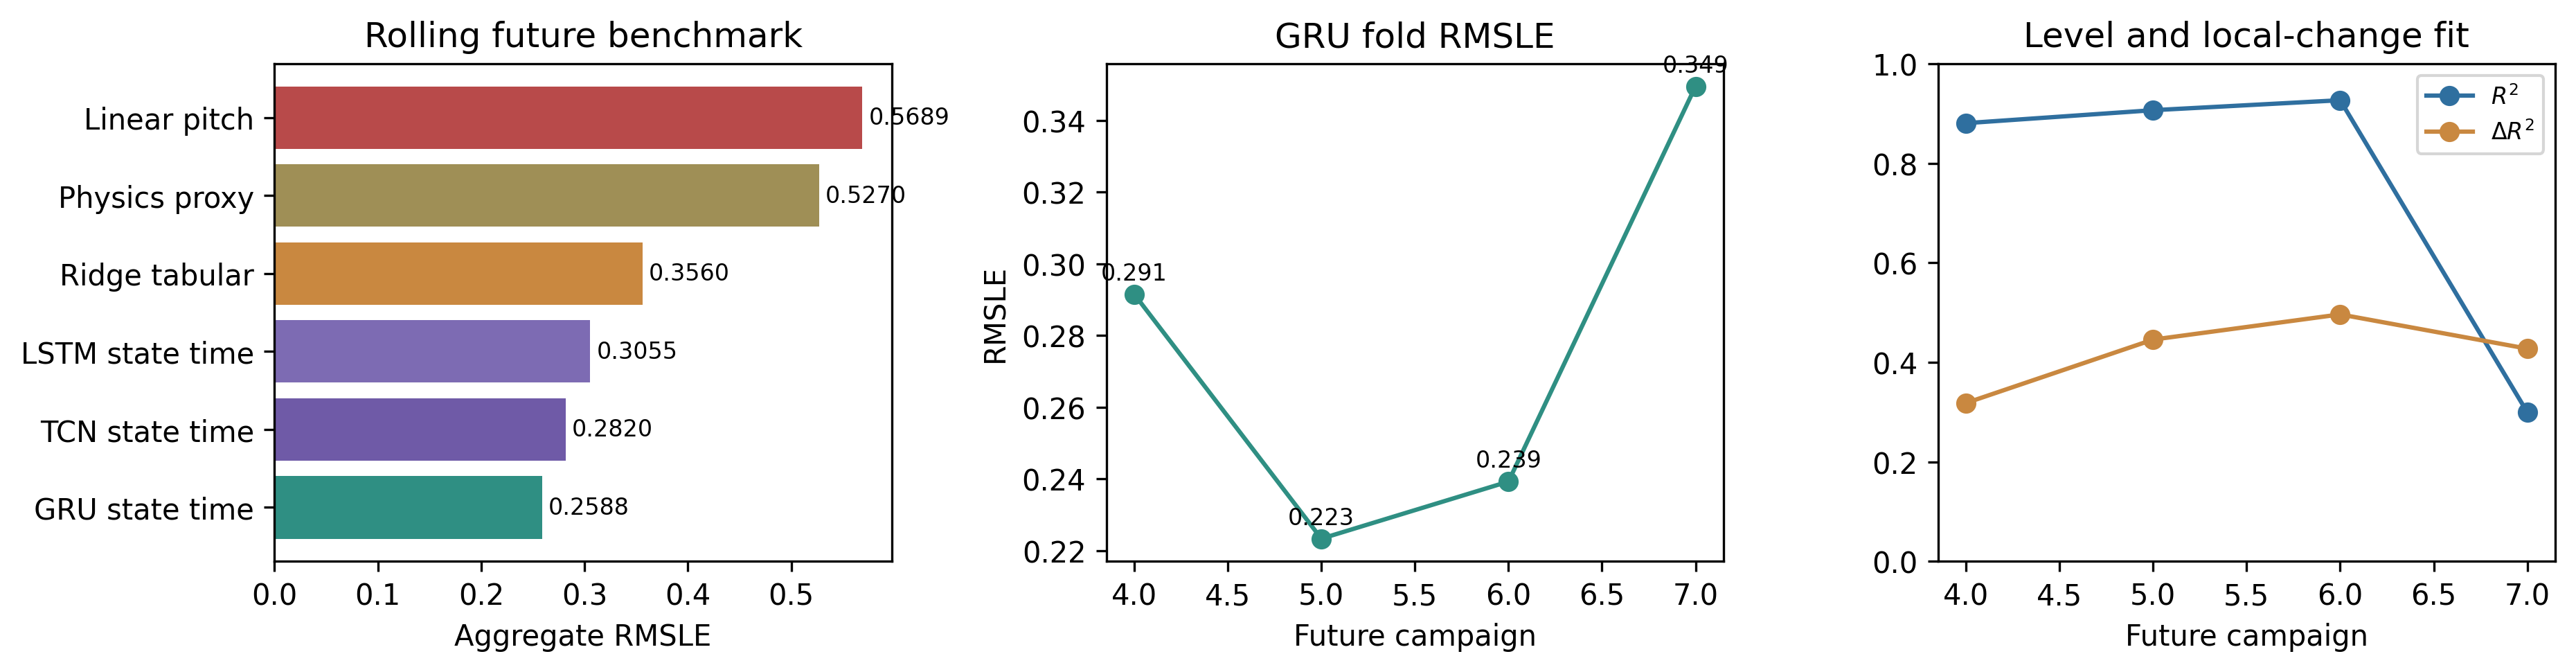
\includegraphics[width=0.68\textwidth]{lncs_figures/rolling_performance_summary.png}
  \caption{Aggregate model comparison and fold level GRU performance; the GRU fold numbers are reported explicitly in Table~\ref{tab:foldgru}.}
  \label{fig:perf}
\end{figure}
\FloatBarrier

\subsection{Future Campaign Performance}

Table~\ref{tab:results} reports aggregate rolling future point estimates. For the selected GRU, flight-cluster bootstrap over 66 future flights gives RMSLE 0.2588, CI [0.2445, 0.2730]; RMSE 22.99\,W, CI [19.87, 26.17]; and $R^2=0.8704$, CI [0.8331, 0.9022].

\begin{table}[!htbp]
\caption{Aggregate C4--C7 rolling future comparison under the same no PWM feature policy.}
\label{tab:results}
\centering
{\small
\begin{tabular}{lcccc}
\toprule
Model & RMSE\,(W) & MAE\,(W) & RMSLE & $R^2$ \\
\midrule
Linear pitch       & 44.51 & 36.00 & 0.5689 & 0.5143 \\
Physics proxy      & 45.52 & 35.72 & 0.5270 & 0.4919 \\
Ridge tabular      & 35.78 & 25.96 & 0.3560 & 0.6861 \\
LSTM state time    & 28.04 & 19.91 & 0.3055 & 0.8073 \\
TCN state time     & 29.32 & 23.70 & 0.2820 & 0.7893 \\
GRU state time     & \textbf{22.99} & \textbf{16.78} & \textbf{0.2588} & \textbf{0.8704} \\
\bottomrule
\end{tabular}
}
\end{table}

The aggregate comparison is not a simple victory claim. GRU has the best RMSLE, RMSE, and $R^2$, but Linear pitch and the physics proxy show the value and limits of transparent references, Ridge benefits from histories, and TCN remains competitive with aggregate RMSLE 0.2820 versus GRU 0.2588.

Table~\ref{tab:foldgru} shows the main stress case. C4--C6 have RMSLE 0.2234--0.2915 and $R^2>0.8806$, whereas C7 reaches RMSE 54.32\,W, RMSLE 0.3494, and $R^2=0.2996$. Modest $\Delta R^2=0.3182$--0.4962 indicates that level behavior is learned more reliably than local spikes or maneuvers. C7's CI [0.3349,0.3599] reflects four high-error flights, so the aggregate GRU result must be read with C7 as a serious failure mode.

\begin{table}[!htbp]
\caption{Fold level selected GRU performance on future campaigns.}
\label{tab:foldgru}
\centering
{\small
\begin{tabular}{lccccccc}
\toprule
Campaign & RMSE\,(W) & MAE\,(W) & RMSLE & RMSLE 95\% CI & $R^2$ & $\Delta R^2$ \\
\midrule
C4 & 21.66 & 17.25 & 0.2915 & [0.2669, 0.3160] & 0.8806 & 0.3182 \\
C5 & 19.24 & 14.71 & 0.2234 & [0.2108, 0.2367] & 0.9066 & 0.4456 \\
C6 & 17.33 & 12.93 & 0.2393 & [0.2238, 0.2542] & 0.9267 & 0.4962 \\
C7 & 54.32 & 48.20 & 0.3494 & [0.3349, 0.3599] & 0.2996 & 0.4273 \\
\bottomrule
\end{tabular}
}
\end{table}

Figure~\ref{fig:perf} visualizes Tables~\ref{tab:results}--\ref{tab:foldgru}: the recurrent baseline is strong in aggregate, while C7 prevents overclaiming.
\FloatBarrier

\subsection{Leakage Controls and Residual Structure}

Figure~\ref{fig:auditdiagnostics} consolidates audit checks. Panel~(a) contrasts valid rolling validation with an invalid random-row reference, which leaks similar timestamps from the same flights/campaigns across the split. Panels~(b)--(c) show good level tracking but heteroscedastic, heavy-tailed residuals and transition errors. This explains why aggregate metrics can look acceptable while maneuvers remain difficult, motivating first-difference $R^2$ and future physics-informed or environmental inputs.

\begin{figure}[!htbp]
  \centering
  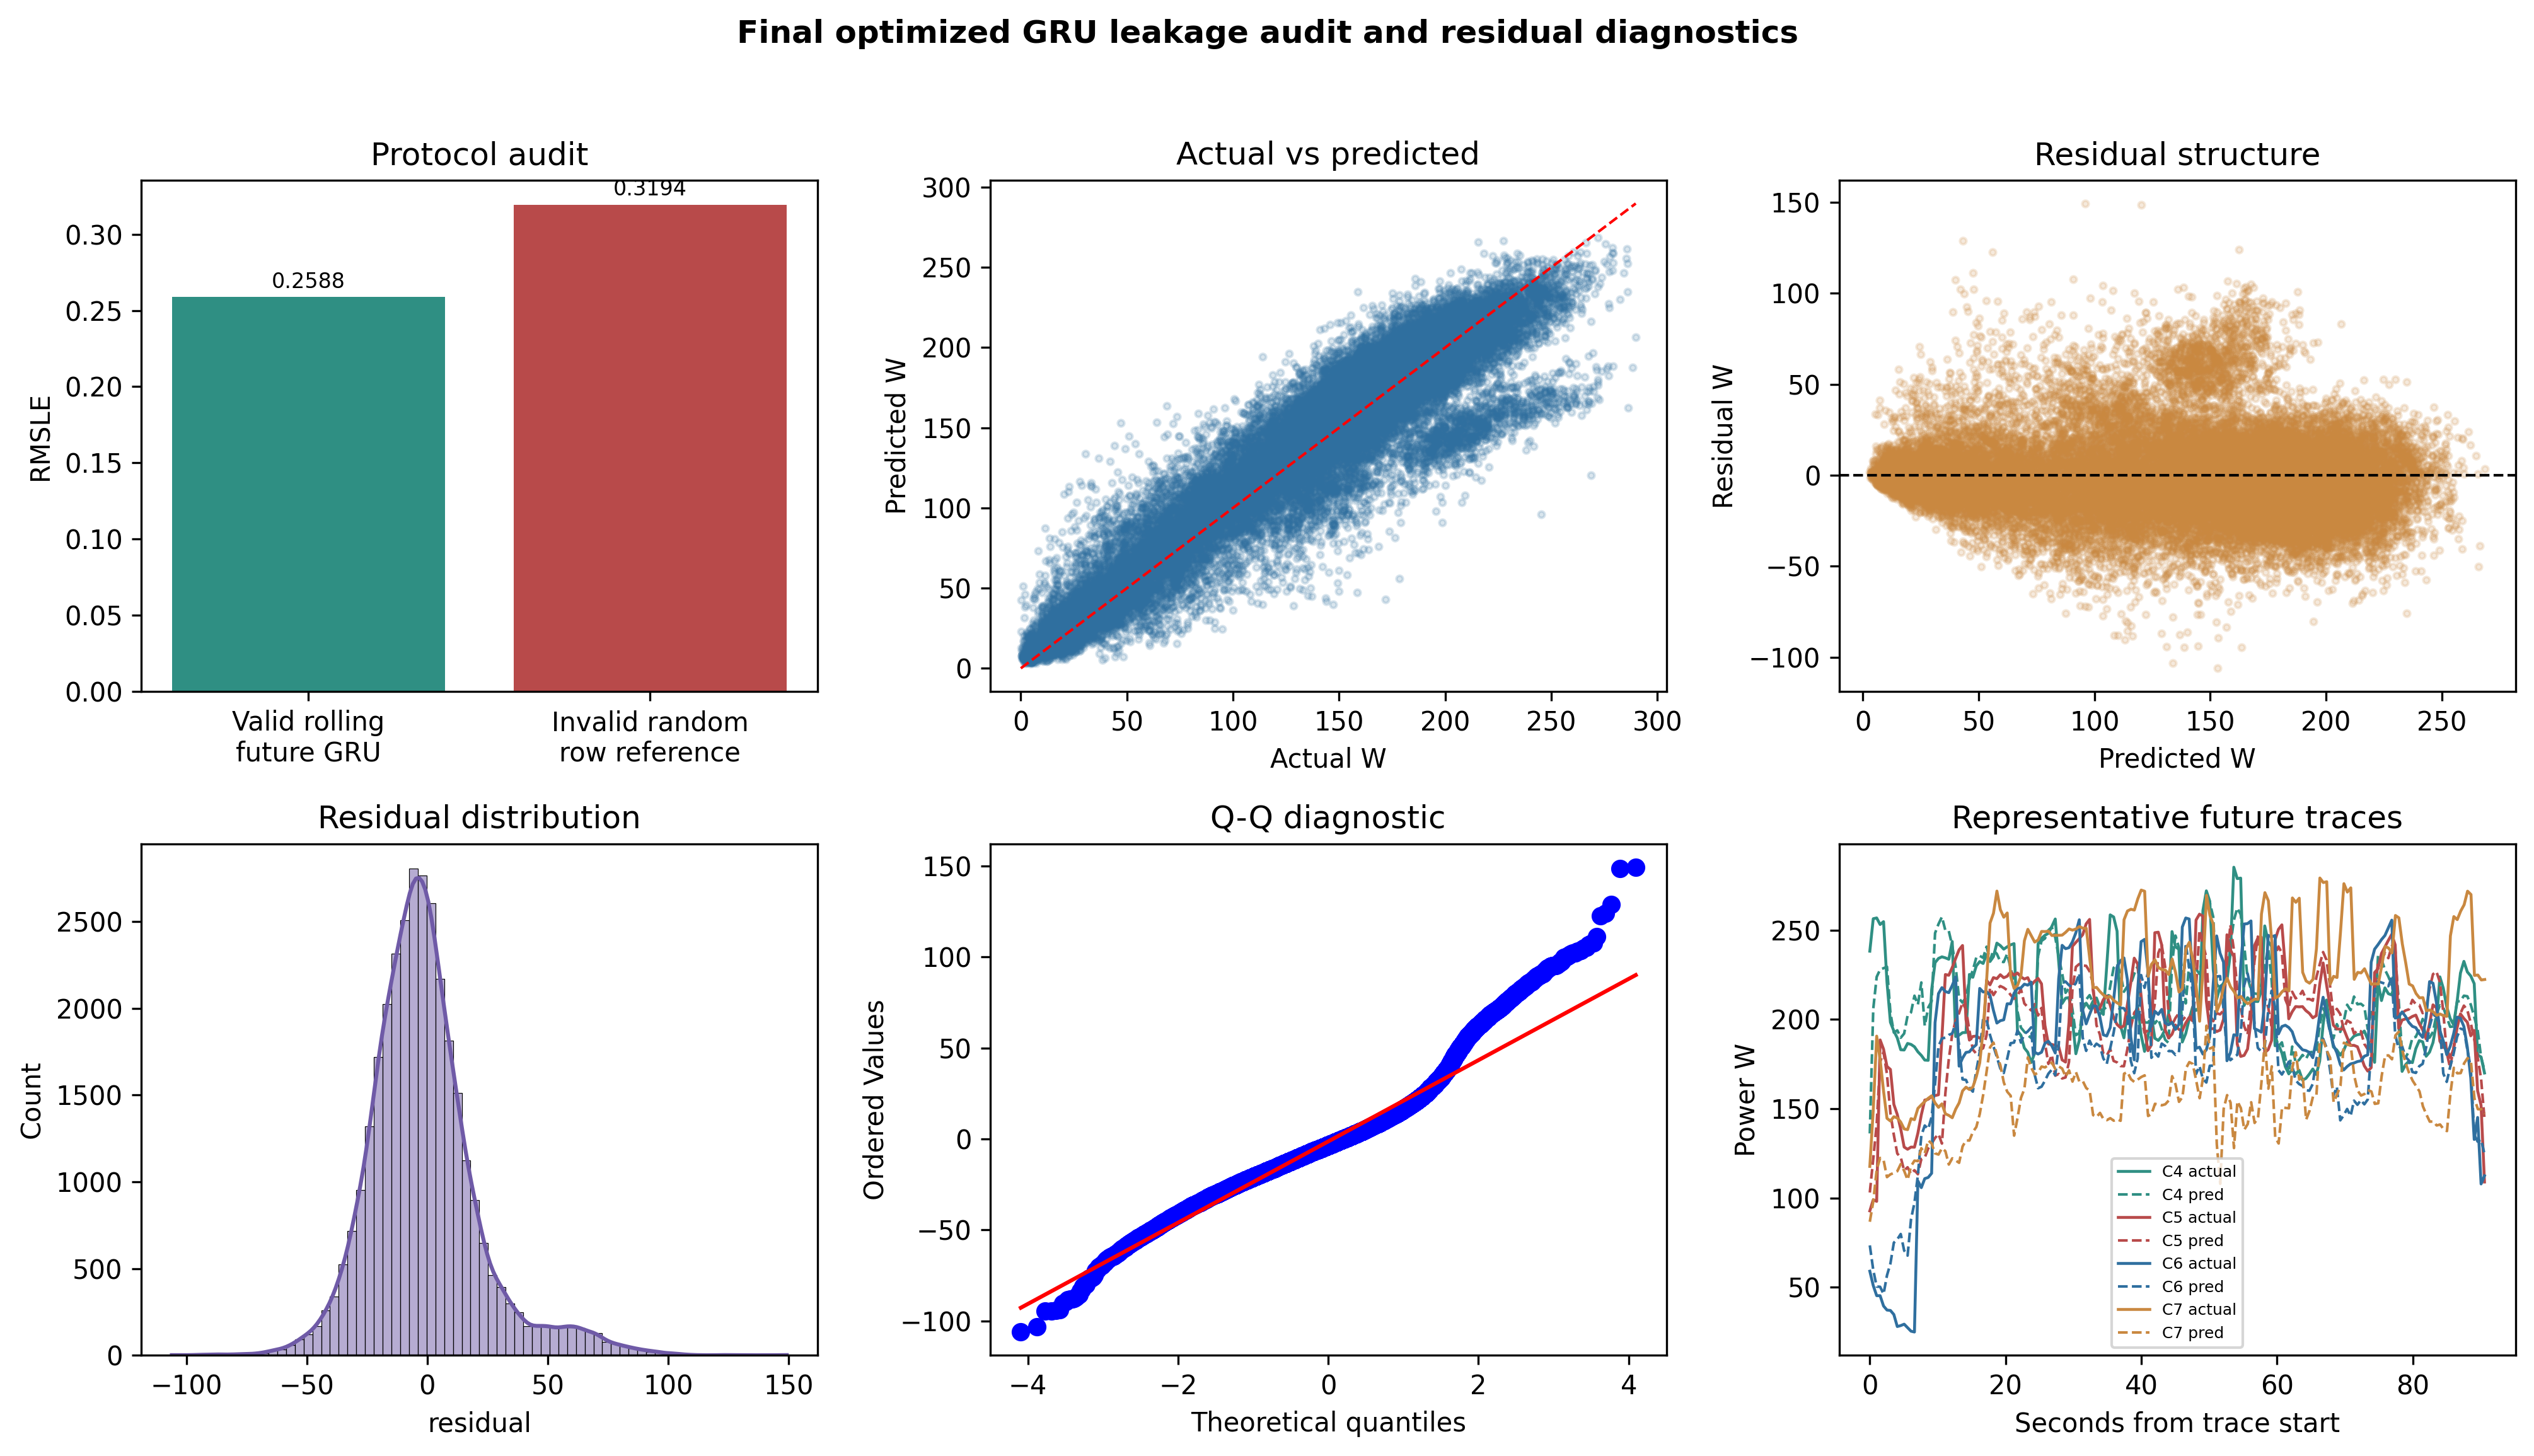
\includegraphics[width=0.65\textwidth]{lncs_figures/tsec_audit_diagnostics_combined.png}
  \caption{Integrated audit and diagnostic visualization for the final GRU. Panel~(a) compares the valid rolling future campaign protocol with an invalid random row reference. Panel~(b) reports actual versus predicted behavior, residual scatter, residual distribution, and Q--Q behavior. Panel~(c) shows representative future campaign traces.}
  \label{fig:auditdiagnostics}
\end{figure}
\FloatBarrier

\newpage
\subsection{Flight-Level Energy and Preliminary Attribution Evidence}

The final stage uses the same held-out GRU predictions for two secondary diagnostics: flight-level energy indicators and preliminary attribution. Algorithm~\ref{alg:smartcityedge} formalizes the workflow, and Fig.~\ref{fig:deployaudit} shows the directly supported evidence layers.

\begin{algorithm}[H]
\scriptsize
\caption{No-PWM GRU flight-level energy audit.}
\label{alg:smartcityedge}
\begin{algorithmic}[1]
\REQUIRE campaigns $C_{1:7}$, cleaned telemetry $\mathcal{D}$, no-PWM features $\mathcal{S}$, GRU family $f_\theta$, SHAP background $\mathcal{B}$
\ENSURE rolling predictions $\hat{P}$, flight energy $E$, watch list $W$, uncertainty summary $U$, SHAP reasons $\phi$
\STATE $\mathcal{D}_{\text{clean}} \leftarrow \text{Clean}(\mathcal{D})$; remove incomplete flights and nonpositive power rows
\STATE $X \leftarrow \text{Window}(\mathcal{D}_{\text{clean}}, \mathcal{S}, 64)$ with only causal samples $t - d \cdot k \le t$
\FOR{rolling split $(C_{1:r}, C_{r+1})$, $r \in \{3,\ldots,6\}$} \STATE train $f_\theta$ on past campaigns only \ENDFOR
\STATE $\hat{P}_t \leftarrow \exp(f_\theta(X_t)) - 1$ and $E_f \leftarrow (1/3600)\sum_{t \in f} \hat{P}_t \cdot \Delta t$ for future flights
\STATE $\tau \leftarrow \mathrm{median}\{E_f : f \in C_{1:3}\} = 10.1057\,\text{Wh}$;\quad $W \leftarrow \{f \in C_{4:7} : E_f > \tau\}$
\STATE $U \leftarrow$ flight error quantiles and watch-list confusion counts
\STATE Select audited GRU $f_{\theta^*}$ by rolling RMSLE
\STATE Compute $\phi \leftarrow \text{GradientSHAP}(f_{\theta^*}, \mathcal{B}, X_{C4:C7})$ across all future flights
\STATE Render Fig.~\ref{fig:deployaudit} from $(E, W, U, \phi)$ and return the human readable audit
\end{algorithmic}
\end{algorithm}

\begin{figure}[!htbp]
  \centering
  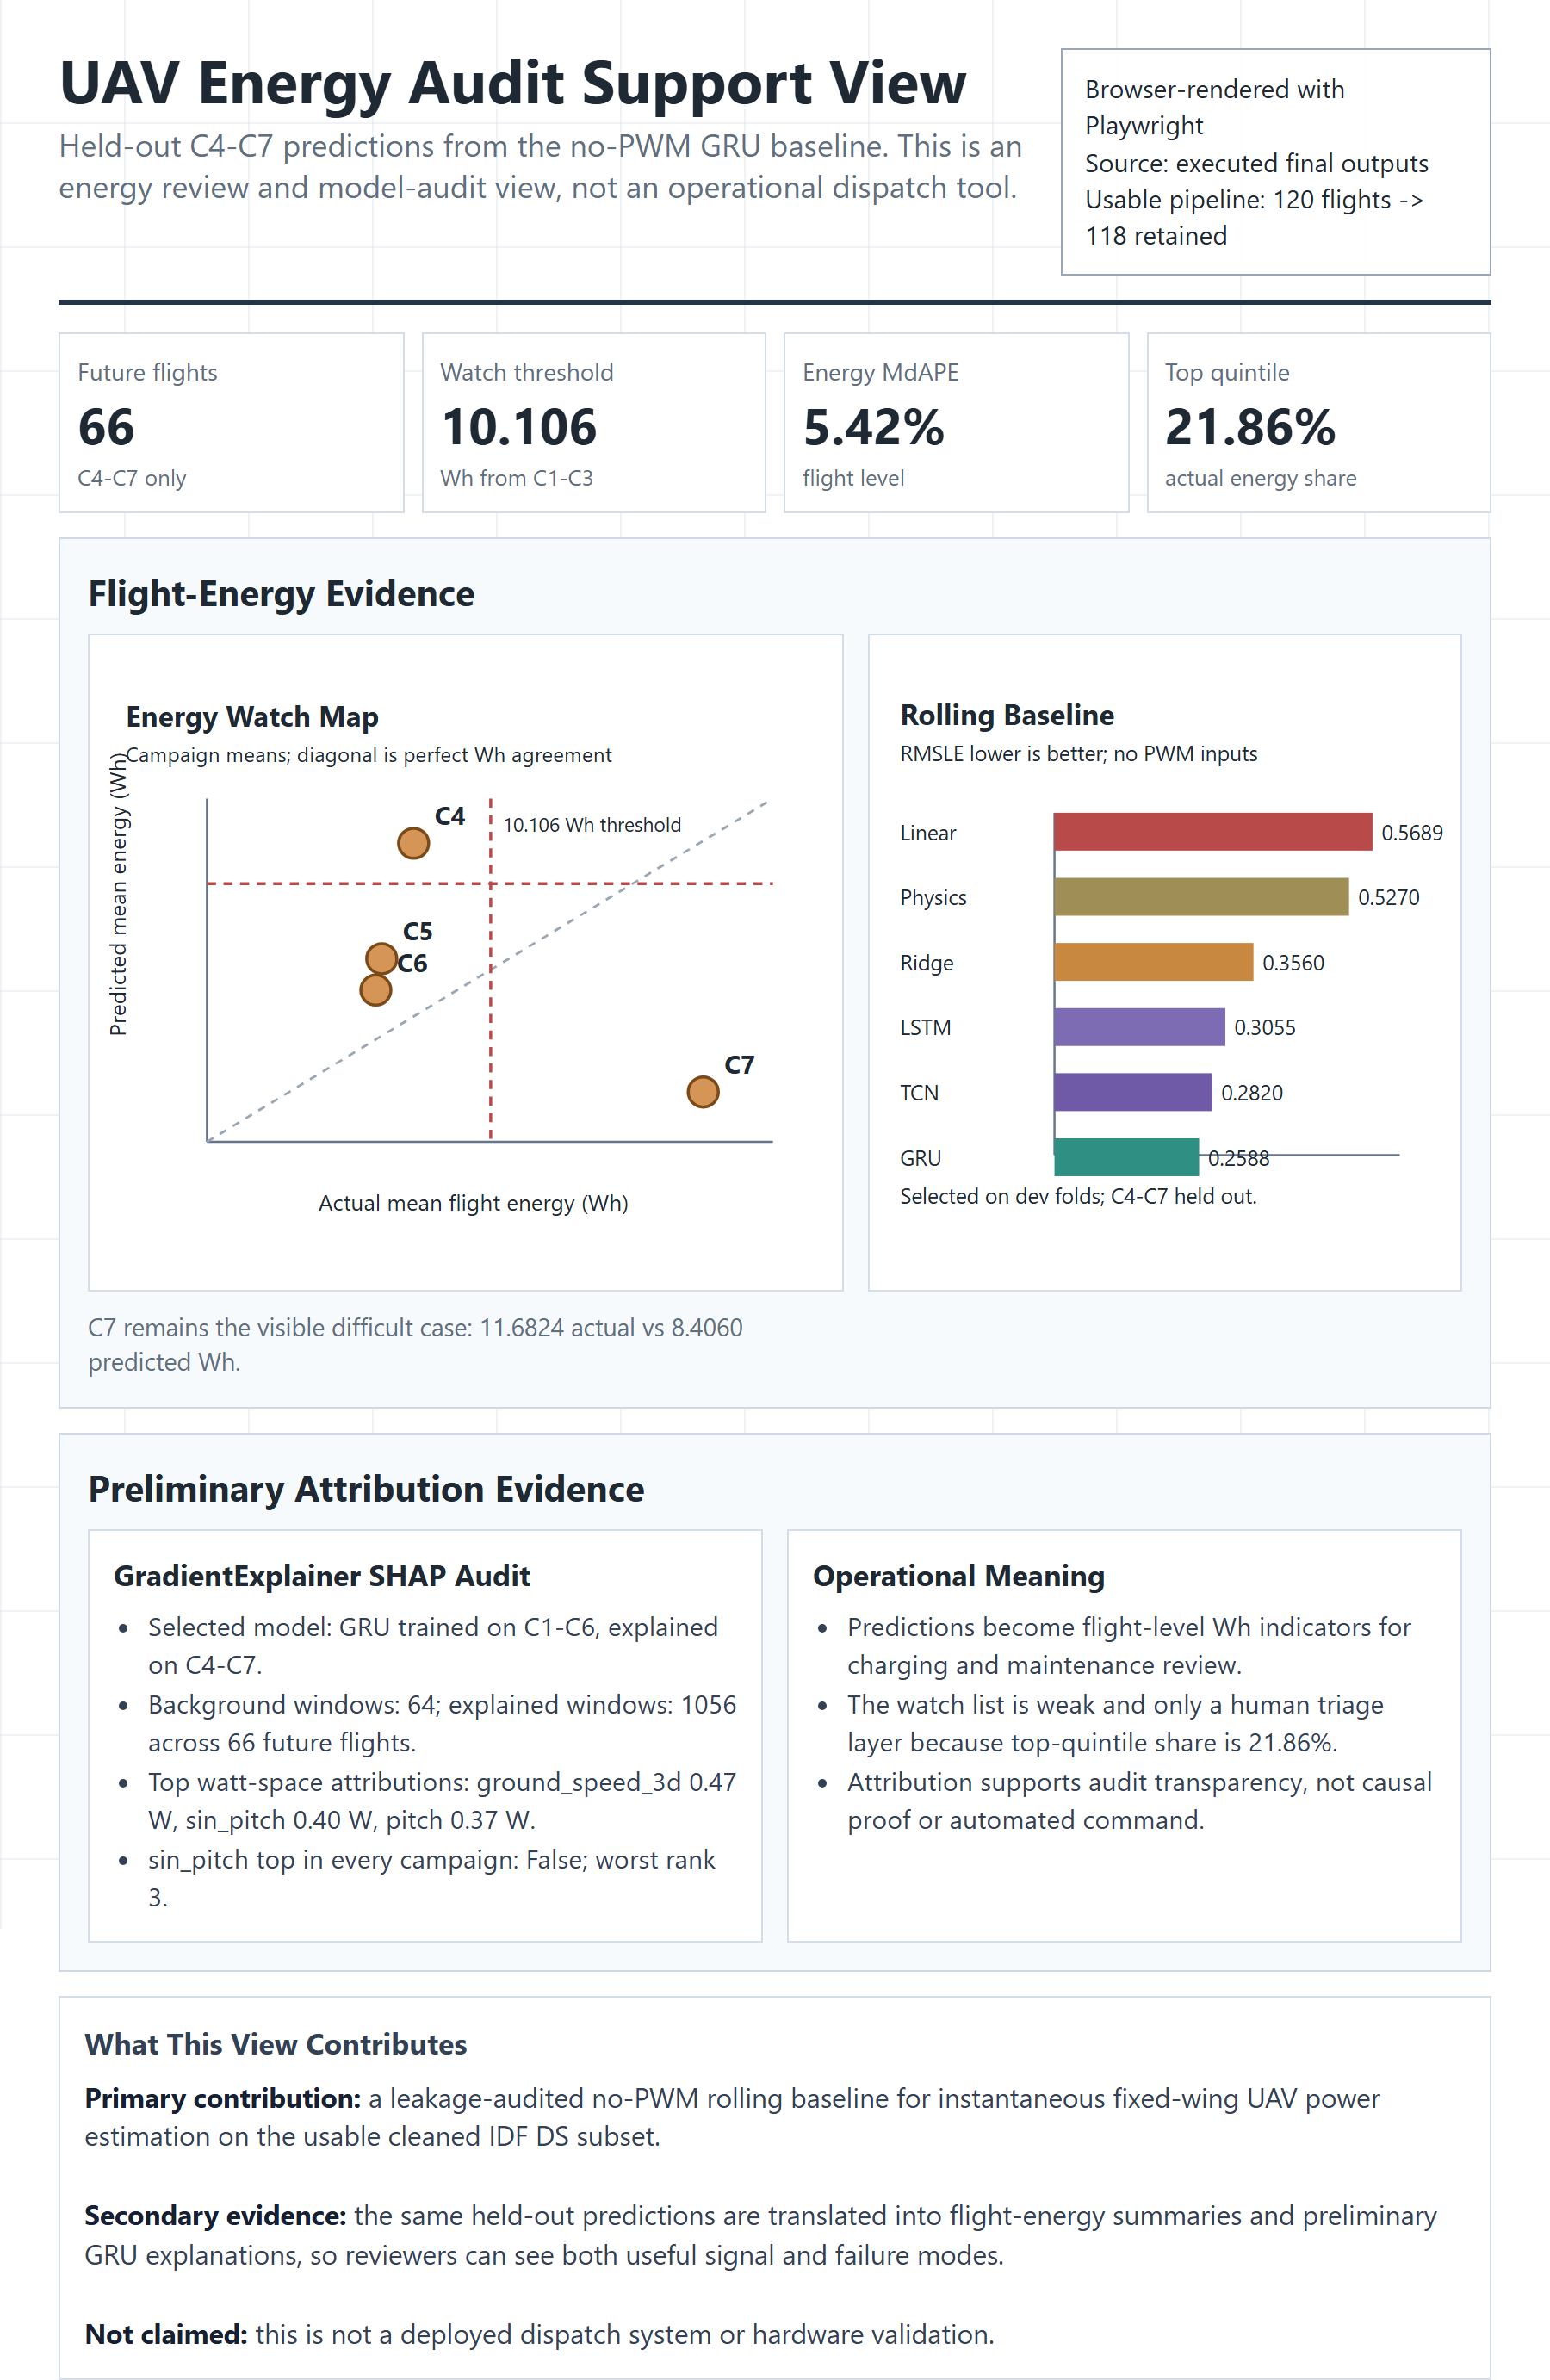
\includegraphics[width=0.82\textwidth]{lncs_figures/smartcity_management_playwright.png}
  \caption{UAV energy audit view rendered from executed final outputs: held out flight energy review, baseline context, preliminary attribution notes, and explicit limitations. The watch-list performance is weak and supports human triage only, not automated dispatch.}
  \label{fig:deployaudit}
\end{figure}

\subsubsection{Flight-level energy evidence.}
Flight energy is $E_f=(1/3600)\sum_t P_f(t)\Delta t_f$ Wh using each flight's median sampling interval. The audit covers 66 future flights from C4--C7 with fixed early-campaign watch threshold 10.1057\,Wh. Future median actual/predicted energy is 9.4221/9.5138\,Wh, mean absolute energy error is 0.7234\,Wh, MdAPE is 5.4231\%, and rank Spearman is 0.2205, consistent with useful magnitude estimates but weak ordering under C7 underprediction. When C7 is excluded, Spearman $\rho$ increases to 0.4629, confirming that late-campaign shift is a major source of rank degradation, although C4--C6 ranking remains only moderate. Absolute energy error has median 0.4743\,Wh, 90th percentile 1.3068\,Wh, and 95th percentile 2.7165\,Wh. Watch-list counts are TP\,=\,4, FP\,=\,9, FN\,=\,5, TN\,=\,48, so precision is 30.8\% versus a 13.6\% positive base rate: better than random but too noisy for automatic dispatch. The top predicted quintile contains 21.8612\% of realized future energy, only 1.8612 points above an unranked 20\% share. Table~\ref{tab:ops} scores the same 66 C4--C7 flights at three thresholds; 10.1057\,Wh remains primary because it is fixed from C1--C3, while 9.0\,Wh illustrates a lower-review threshold for higher recall.

\begin{table}[!htbp]
\caption{Three operating thresholds for flight-level watch-list review.}
\label{tab:ops}
\centering
{\scriptsize
\begin{tabular}{lcccc}
\toprule
Threshold & TP & FP & Precision & Recall \\
\midrule
9.000\,Wh & 38 & 15 & 0.717 & 0.809 \\
10.1057\,Wh & 4 & 9 & 0.308 & 0.444 \\
11.000\,Wh & 0 & 3 & 0.000 & 0.000 \\
\bottomrule
\end{tabular}
}
\end{table}

\subsubsection{Preliminary attribution evidence for flight-level review.}
GradientExplainer is computed on the selected GRU trained on C1--C6 and explained on all 66 C4--C7 future flights, using 64 background windows and 16 explanation windows per flight (1056 windows), replacing an earlier 528-window audit with the improved final setup. Since the GRU predicts $\log(1+P)$, local attributions are mapped approximately to watts by multiplying by $\exp(\hat{y})$. Flight-cluster bootstrap gives the leading watt-space mean $|\mathrm{SHAP}|$: \texttt{ground\_speed\_3d} 0.466\,W [0.431, 0.504], \texttt{sin\_pitch} 0.399\,W [0.386, 0.410], \texttt{pitch} 0.373\,W [0.360, 0.385], and \texttt{speed\_horizontal} 0.372\,W [0.344, 0.402]. These small averaged values support ranking, not additive flight-energy accounting. They also have the expected physical reading: speed and attitude variables dominate because the no-PWM feature policy leaves aerodynamic state, rather than actuator demand, as the main observable pathway.

Permutation importance on the same windows gives baseline sampled RMSE 19.12\,W; permuting \texttt{log\_elapsed\_s}, \texttt{sin\_pitch}, \texttt{air\_rho}, and \texttt{pitch} increases RMSE by 18.64, 14.24, 7.79, and 7.45\,W. It agrees that attitude and air density matter but makes time context the strongest perturbation, so attribution remains preliminary model-audit evidence.

Cross-campaign stability is more informative than a single global rank. The feature \texttt{sin\_pitch} is top only in C5, rank 3 in C4, rank 2 in C6, and rank 2 in C7 where \texttt{air\_rho} leads. It is important but not invariant. This non-invariance is itself an important result: the model's explanation shifts when the operating regime shifts, which is consistent with the C7 performance drop and argues against presenting any one state variable as a universal driver. The most recent 0--5\,s still accounts for 70.26\% of watt-space attribution mass.

\FloatBarrier

%------------------------------------------------------------------------
\section{Discussion}

The state time GRU is credible only under some future-campaign conditions: C4--C6 are modeled reasonably well, while C7 is a serious failure mode. This does not make PWM or electrical measurements unimportant; it shows what remains possible in incomplete, heterogeneous, or state-only telemetry settings.

The recurrent comparison is informative but not uniform. GRU improves aggregate C4--C7 and C5--C6 RMSLE, but TCN is lower on C4 and C7, including C7 RMSLE 0.2666 versus GRU 0.3494. The selected two-layer GRU is chosen only from development rolling splits.

C7 is the main limitation, not a side note. With only four flights we avoid a population-level shift claim, but the stress case is clear: $R^2$ drops to 0.2996 and RMSE rises to 54.32\,W. Relative to C1--C6, C7 has lower air density (1.1239 vs. 1.1622\,kg/m$^3$, SMD\,$-6.19$), more negative pitch ($-0.0565$ vs. 0.0271\,rad, SMD\,$-6.04$), higher actual power (166.00 vs. 134.49\,W, SMD\,3.13), and larger residuals (46.57 vs. $-4.33$\,W, SMD\,7.51). The model predicts lower mean power in C7 than before (119.43 vs. 138.82\,W, SMD\,$-2.64$), while path length, horizontal distance, and altitude range are similar. The pattern is therefore closer to environment-attitude-calibration shift than route length.

The lightweight adaptation test freezes the GRU and fits only $\log(1+\hat{P}')=a\log(1+\hat{P})+b$ on the first one or two labeled C7 flights. With flight 117 for adaptation and 118--120 for evaluation, RMSLE, RMSE, and $R^2$ improve from 0.3458, 53.09\,W, and 0.3144 to 0.1750, 18.64\,W, and 0.9155. With flights 117--118 for adaptation and 119--120 for evaluation, they improve from 0.3389, 51.17\,W, and 0.3468 to 0.1822, 18.69\,W, and 0.9129. This is preliminary because C7 has four flights, but it shows that early campaign supervision can substantially reduce the gap. The result reframes C7 from a simple limitation into a concrete future direction: the base sequence representation appears useful, while its output calibration is sensitive to campaign-level environment and attitude shift.

A minimum field-use guard is therefore: compare flight-level SMDs for power proxies, air density, pitch, and dynamic pressure against the training reference; if any $|\mathrm{SMD}|>2.0$, or if predicted energy lies within the 2.7165\,Wh error band around the watch threshold, flag for human review and recalibration. C7 would trigger this guard.

The intended operational interpretation is deliberately conservative. A future energy-audit system would attach three qualifiers before any planning action: the campaign-shift guard, the flight-level error band, and the attribution summary. A flight near the threshold or under a C7-like warning would be sent to review or recalibration rather than used as an unqualified dispatch rule. The attribution stability check serves the same purpose: \texttt{sin\_pitch} is important but not invariant, so campaign-aware monitoring is more defensible than a single global driver claim.

Design boundaries remain. \texttt{t\_sec} would be leakage if it encoded future duration, target history, or route identity; here it is only current elapsed time and fixed cycles. Remaining errors likely reflect unobserved gusts, payload, configuration, battery health, controller modes, and campaign shifts. The results should not be generalized to multi-platform or multi-mission settings without renewed validation. Open extensions include attention/probabilistic models, online adaptation, calibrated uncertainty, broader attribution audits, feature-group ablations, and stronger physics-informed baselines.

%------------------------------------------------------------------------
\section{Conclusion}

The paper contributes a reproducible pipeline for high-frequency UAV telemetry: a leakage-audited task, causal state time features, future-campaign validation, and diagnostics rather than a single leaderboard score. Within the IDF DS neural-prediction gap~\cite{garcia2026idfds}, it demonstrates no-PWM instantaneous power prediction from vehicle state history alone.

For fleet energy monitoring, the output is a review signal rather than an automatic dispatch command. A manager of an urban UAV inspection fleet receives, after each route, predicted Wh, watch status relative to the 10.1057\,Wh threshold, attribution notes, and the 2.7165\,Wh error band. That band maps to about 2.7 minutes of charging-time uncertainty at 60\,W, or 5.4 minutes at 30\,W, giving scheduling slack and triggering review for C7-like shift warnings. This charging-time calculation is separate from $\Delta R^2$, which remains a local-change diagnostic and is only about 0.32--0.50 across future campaigns. In such a workflow the model does not decide dispatch; it prioritizes which flights deserve battery-log inspection, charger-buffer adjustment, or recalibration before the next route batch.

This scenario is intentionally modest: rolling accuracy, preliminary attribution, uncertainty summaries, and flight-level aggregation all come from the same leakage-audited protocol.

The reporting boundary is equally important. The study does not claim an edge-ready controller, calibrated uncertainty model, or complete aerodynamic estimator. Its narrower claim is that, under a fixed no-PWM contract and strict campaign chronology, a recurrent state-history model can estimate power well in C4--C6-like future campaigns while C7 exposes a concrete shift problem. Follow-up work should repeat the lightweight adaptation test on larger shifts and extend attribution with grouped perturbations, campaign-specific uncertainty, and physical covariates.

The selected GRU achieved aggregate RMSLE 0.2588 and $R^2=0.8704$ under strict rolling validation. The result supports no-PWM estimation under C4--C6-like conditions, but C7 shows the task is not solved and campaign shift can dominate. Future work should improve shift robustness, add legitimate weather/payload metadata, calibrate uncertainty, and compare attention, probabilistic, and physics-informed models without reintroducing leakage.

\paragraph{Acknowledgements.}
The authors thank the IDF DS dataset creators for releasing the fixed wing UAS telemetry benchmark used in this study. AI-assisted language editing tools were used for language polishing and formatting checks only; all scientific claims, experimental design, code execution, data analysis, results, and conclusions were produced and verified by the authors.

%------------------------------------------------------------------------
\begin{thebibliography}{99}

\bibitem{shakhatreh2019survey}
Shakhatreh, H., et al.: Unmanned aerial vehicles (UAVs): A survey on civil applications and key research challenges. \textit{IEEE Access} \textbf{7}, 48572--48634 (2019). \href{https://arxiv.org/abs/1805.00881}{arXiv:1805.00881}

\bibitem{zeng2017energy}
Zeng, Y., Zhang, R.: Energy-efficient UAV communication with trajectory optimization. \textit{IEEE Transactions on Wireless Communications} \textbf{16}(6), 3747--3760 (2017). \href{https://arxiv.org/abs/1608.01828}{arXiv:1608.01828}

\bibitem{mozaffari2019tutorial}
Mozaffari, M., et al.: A tutorial on UAVs for wireless networks: Applications, challenges, and open problems. \textit{IEEE Communications Surveys \& Tutorials} \textbf{21}(3), 2334--2360 (2019). \href{https://arxiv.org/abs/1803.00680}{arXiv:1803.00680}

\bibitem{hayat2016survey}
Hayat, S., Yanmaz, E., Muzaffar, R.: Survey on unmanned aerial vehicle networks for civil applications: A communications viewpoint. \textit{IEEE Communications Surveys \& Tutorials} \textbf{18}(4), 2624--2661 (2016). \href{https://mobile.aau.at/publications/hayat-2016-COMST-surveyUAV.pdf}{open PDF}

\bibitem{garcia2026idfds}
Garc\'ia-Gasc\'on, C., et al.: An open benchmark dataset for machine learning and intelligent trajectory optimization in fixed-wing unmanned aerial systems. \textit{Scientific Data} \textbf{13}, 364 (2026). \href{https://doi.org/10.1038/s41597-026-06716-3}{doi:10.1038/s41597-026-06716-3}

\bibitem{garcia2025zenodo}
Garc\'ia Gasc\'on, C.: Fixed-Wing UAS Telemetry Benchmark (IDF\_DS): 240 Flights for ML and Intelligent Trajectory Optimization, version v1.0. Zenodo (2025). \href{https://doi.org/10.5281/zenodo.16992976}{doi:10.5281/zenodo.16992976}

\bibitem{yaacoub2020security}
Yaacoub, J.P., et al.: Security analysis of drones systems: Attacks, limitations, and recommendations. \textit{Internet of Things} \textbf{11}, 100218 (2020). \href{https://doi.org/10.1016/j.iot.2020.100218}{doi:10.1016/j.iot.2020.100218}

\bibitem{lundberg2017shap}
Lundberg, S.M., Lee, S.-I.: A unified approach to interpreting model predictions. In: \textit{Advances in Neural Information Processing Systems} 30, pp.~4765--4774 (2017). \href{https://arxiv.org/abs/1705.07874}{arXiv:1705.07874}

\bibitem{arrieta2020xai}
Arrieta, A.B., et al.: Explainable artificial intelligence (XAI): Concepts, taxonomies, opportunities and challenges toward responsible AI. \textit{Information Fusion} \textbf{58}, 82--115 (2020). \href{https://doi.org/10.1016/j.inffus.2019.12.012}{doi:10.1016/j.inffus.2019.12.012}

\bibitem{difranco2016coverage}
Di Franco, C., Buttazzo, G.: Coverage path planning for UAVs photogrammetry with energy and resolution constraints. \textit{Journal of Intelligent \& Robotic Systems} \textbf{83}, 445--462 (2016). \href{https://doi.org/10.1007/s10846-016-0348-x}{doi:10.1007/s10846-016-0348-x}

\bibitem{abeywickrama2018access}
Abeywickrama, H.V., et al.: Comprehensive energy consumption model for unmanned aerial vehicles, based on empirical studies of battery performance. \textit{IEEE Access} \textbf{6}, 58383--58394 (2018). \href{https://www.researchgate.net/publication/328188643_Comprehensive_Energy_Consumption_Model_for_Unmanned_Aerial_Vehicles_Based_on_Empirical_Studies_of_Battery_Performance}{public full text}

\bibitem{gora2022ml}
G\'ora, K., et al.: Machine learning in creating energy consumption model for UAV. \textit{Energies} \textbf{15}(18), 6810 (2022). \href{https://doi.org/10.3390/en15186810}{doi:10.3390/en15186810}

\bibitem{zhang2021models}
Zhang, J., et al.: Energy consumption models for delivery drones: A comparison and assessment. \textit{Transportation Research Part D} \textbf{90}, 102668 (2021). \href{https://doi.org/10.1016/j.trd.2020.102668}{doi:10.1016/j.trd.2020.102668}

\bibitem{bai2018tcn}
Bai, S., Kolter, J.Z., Koltun, V.: An empirical evaluation of generic convolutional and recurrent networks for sequence modeling. \textit{arXiv preprint} arXiv:1803.01271 (2018). \href{https://arxiv.org/abs/1803.01271}{arXiv:1803.01271}

\bibitem{kaufman2012leakage}
Kaufman, S., et al.: Leakage in data mining: formulation, detection, and avoidance. \textit{ACM Transactions on Knowledge Discovery from Data} \textbf{6}(4), Article 15 (2012). \href{https://doi.org/10.1145/2382577.2382579}{doi:10.1145/2382577.2382579}

\bibitem{bergmeir2018cv}
Bergmeir, C., Hyndman, R.J., Koo, B.: A note on the validity of cross-validation for evaluating autoregressive time series prediction. \textit{Computational Statistics \& Data Analysis} \textbf{120}, 70--83 (2018). \href{https://doi.org/10.1016/j.csda.2017.11.003}{doi:10.1016/j.csda.2017.11.003}

\bibitem{hyndman2006forecast}
Hyndman, R.J., Koehler, A.B.: Another look at measures of forecast accuracy. \textit{International Journal of Forecasting} \textbf{22}(4), 679--688 (2006). \href{https://doi.org/10.1016/j.ijforecast.2006.03.001}{doi:10.1016/j.ijforecast.2006.03.001}

\bibitem{salinas2020deepar}
Salinas, D., et al.: DeepAR: Probabilistic forecasting with autoregressive recurrent networks. \textit{International Journal of Forecasting} \textbf{36}(3), 1181--1191 (2020). \href{https://arxiv.org/abs/1704.04110}{arXiv:1704.04110}

\bibitem{lim2021tft}
Lim, B., et al.: Temporal Fusion Transformers for interpretable multi-horizon time series forecasting. \textit{International Journal of Forecasting} \textbf{37}(4), 1748--1764 (2021). \href{https://arxiv.org/abs/1912.09363}{arXiv:1912.09363}

\bibitem{fawaz2019dlts}
Ismail Fawaz, H., et al.: Deep learning for time series classification: a review. \textit{Data Mining and Knowledge Discovery} \textbf{33}, 917--963 (2019). \href{https://arxiv.org/abs/1809.04356}{arXiv:1809.04356}

\bibitem{hochreiter1997lstm}
Hochreiter, S., Schmidhuber, J.: Long short-term memory. \textit{Neural Computation} \textbf{9}(8), 1735--1780 (1997). \href{https://doi.org/10.1162/neco.1997.9.8.1735}{doi:10.1162/neco.1997.9.8.1735}

\bibitem{cho2014gru}
Cho, K., et al.: Learning phrase representations using RNN encoder-decoder for statistical machine translation. In: \textit{Proceedings of the 2014 Conference on Empirical Methods in Natural Language Processing (EMNLP)}, pp.~1724--1734. Association for Computational Linguistics (2014). \href{https://doi.org/10.3115/v1/D14-1179}{doi:10.3115/v1/D14-1179}

\bibitem{batty2012smart}
Batty, M., et al.: Smart cities of the future. \textit{The European Physical Journal Special Topics} \textbf{214}, 481--518 (2012). \href{https://doi.org/10.1140/epjst/e2012-01703-3}{doi:10.1140/epjst/e2012-01703-3}

\bibitem{stolaroff2018drone}
Stolaroff, J.K., et al.: Energy use and life cycle greenhouse gas emissions of drones for commercial package delivery. \textit{Nature Communications} \textbf{9}, 409 (2018). \href{https://doi.org/10.1038/s41467-017-02411-5}{doi:10.1038/s41467-017-02411-5}

\end{thebibliography}

\end{document}
